\documentclass[14pt, aspectratio=169]{beamer}

\usetheme{Copenhagen}
\setbeamertemplate{navigation symbols}{} % Esconde as barras de navegação inferiores
\setbeamercovered{transparent}
\setbeamertemplate{headline}{} % Esconde a barra de navegação no topo do documento, relativa às seções

\newcommand{\R}{\mathbb{R}}
\newcommand{\I}{\mathbb{I}}
\newcommand{\Q}{\mathbb{Q}}
\newcommand{\Z}{\mathbb{Z}}
\newcommand{\N}{\mathbb{N}}

\newtheorem{theo}{Teorema}
\newtheorem{ex}{Exemplo}

\input{pacotes.tex}

\title{Conjuntos numéricos}
\subtitle{Pré-cálculo}
\author{Prof. Dr. Márcio Leandro Gonçalves}
\date{\today}
\institute{PUC Minas - Poços de Caldas}

\begin{document}

\begin{frame}
\maketitle 
\end{frame}

\begin{frame}[allowframebreaks]{Principais conjuntos}
\begin{itemize}
    \item Números naturais: $\N = \{ 0,1,2,3, \cdots \}$
    \item Números inteiros: $\Z = \{\cdots, -3, -2, -1, 0, 1, 2, 3, \cdots \}$ 
    \begin{itemize}
        \item O conjunto dos inteiros é uma ampliação do conjuntos dos naturais.
        \item É formado pela união dos naturais com os negativos ($\mathbb{Z} = \{ \cdots, -3, -2, -1\} \cup \N$).
        \item Note que $\N \subset \Z$.
    \end{itemize}

    \vspace{5.0cm}
    
    \item Números racionais: $\Q = \left\{ \dfrac{a}{b} \mid a,b \in \Z \text{ e } b \neq 0 \right\}$
    \begin{itemize}
        \item Um número $x$ é dito racional se existem dois números inteiros $a$ e $b$ ($b \neq 0$) de modo que $x$ é o resultado da divisão de $a$ por $b$.
        \item Em outras palavras, \emph{se é fração ou pode ser escrito como uma fração então o número é racional}.
        \item Observe que $\Z \subset Q$.
    \end{itemize}

    \vspace{5.0cm}

    \item Números irracionais: $\I$.
    \begin{itemize}
        \item Um número irracional é aquele que \emph{não pode} ser obtido pela divisão de dois números inteiros.
        \item Em outras palavras, \emph{não pode ser escrito como uma fração.}
        \item Exemplos:
            \begin{itemize}
                \item $\pi = 3,141592\ldots$
                \item $e = 2,718281828\ldots$
                \item $\phi = 1,618033989\ldots$
                \item $\sqrt{2} = 1,41421356\ldots$
            \end{itemize}
    \end{itemize}

    \vspace{5.0cm}

    \item Números reais: $\R = \Q \cup \I$.
    \begin{itemize}
        \item Esse conjunto é uma expansão do conjunto dos números racionais que engloba não só os inteiros e fracionários, positivos e negativos, mas também todos os números irracionais.
        \item Reta real: \\ 
        \vspace{0.25cm}
        \begin{tikzpicture}
            % x-axis
            \draw[<->] (-5,0) -- (5,0);

            \foreach \i in {-4,-3,...,4} % points on line
            \fill [blue] (\i,0) circle (0.6 mm)
            node[below=2pt, black] {$\i$};

            \draw[fill=black] (5/2, 0) circle (0.6 mm)
            node[below=4pt, black] {\scriptsize $\dfrac{5}{2}$};

            \draw[fill=black] ({sqrt(2)}, 0) circle (0.6 mm)
            node[below=4pt, black] {\scriptsize $\sqrt{2}$};
        \end{tikzpicture}
    \end{itemize}

    \vspace{5.0cm}

    \item É evidente que $\N \subset \Z \subset \Q \subset \R$.
\end{itemize}
\end{frame}

\begin{frame}[allowframebreaks]{Observações importantes}

\begin{itemize}
    \item Quando acrescentamos o símbolo $*$ (estrela) num conjunto numérico, estamos indicando que o zero foi excluído do conjunto. 
    
    \item Exemplo: $\Z^* = \{ x \in \Z \mid x \neq 0 \} = \{ \ldots, -2, -1, 1, 2, \ldots \}$
    
    \vspace{5.0cm}
    
    \item Quando acrescentamos o símbolo $+$ (mais) num conjunto numérico, estamos indicando que foram excluídos todos os números negativos do conjunto.

    \item Exemplo: $\Z_+ = \{ x \in \Z \mid x \geq 0 \} = \{0, 1, 2, 3, \ldots \}$

    \vspace{5.0cm}
    
    \item Quando acrescentamos o símbolo $-$ (menos) num conjunto numérico, estamos indicando que foram excluídos todos os números positivos do conjunto.

    \item Exemplo: $\Z_- = \{ x \in \Z \mid x \leq 0 \} = \{\ldots, -3, -2, -1, 0 \}$

    \vspace{5.0cm}
    
    \item Deve-se observar que o número zero é elemento dos conjuntos $\Z_+, \Z_-, \Q_+, \Q_-, \R_+, \R_-$.

    \item Para excluirmos o zero destes conjuntos, devemos usar as seguintes representações: $\Z_+^*, \Z_-^*, \Q_+^*, \Q_-^*, \R_+^*, \R_-^*$.
    
\end{itemize}
    
\end{frame}

\begin{frame}[allowframebreaks]{Intervalos numéricos}
    
\end{frame}

\begin{frame}[allowframebreaks]{Noções de conjuntos}

\begin{itemize}
    \item Conjunto unitário: é aquele formado por um único elemento. 
    
    \item Exemplo: $A = \{ x \in \Z_+ \mid x^2 = 1 \}$ é unitário, pois $A = \{ 1 \}$.

    \vspace{5.0cm}

    \item Conjunto vazio: é aquele que não possui elementos.
    
    \item Notação: $\varnothing$ ou $\{ \}$.
\end{itemize}

\end{frame}

\begin{frame}[allowframebreaks]{Operações de conjuntos}

Reunião de conjuntos:

 \begin{itemize}
    \item Dados dois conjuntos $A$ e $B$, chama-se \emph{união} de $A$ e $B$ conjunto formado pelos elementos que pertencem a $A$ \emph{ou} a $B$.
    \item Simbolicamente: $A \cup B = \{x \mid x \in A \text{ ou } x \in B \}$.
    \item Exemplos: 
        \begin{itemize}
            \item $\{ 1, 2 \} \cup \{ 3, 4 \} = \{ 1, 2, 3, 4 \}$
            \item $\varnothing \cup \{ 3, 4 \} = \{ 3, 4 \}$
        \end{itemize}
\end{itemize}

\vspace{5.0cm}

Interseção de conjuntos:

\begin{itemize}
    \item Dados dois conjuntos $A$ e $B$, chama-se \emph{interseção} de $A$ e $B$ conjunto formado pelos elementos que pertencem a $A$ \emph{e} a $B$.
    \item Simbolicamente: $A \cap B = \{x \mid x \in A \text{ e } x \in B \}$.
    \item Exemplos: 
        \begin{itemize}
            \item $\{ -2, 4, 7 \} \cap \{-4, 2, 7 \} = \{ 7 \}$
            \item $\{ 5, 7 \} \cap \{ 6, 10 \} = \varnothing$
        \end{itemize}
    \item OBS: Quando $A \cap B = \varnothing $ dizemos que $A$ e $B$ são \emph{conjuntos disjuntos}.
    
\end{itemize}

\vspace{5.0cm}

Diferença de conjuntos:

 \begin{itemize}
    \item Dados dois conjuntos $A$ e $B$, chama-se \emph{diferença} entre $A$ e $B$ conjunto formado pelos elementos que pertencem a $A$ \emph{e não} a $B$.
    \item Simbolicamente: $A - B = \{x \mid x \in A \text{ e } x \notin B \}$.
    \item Exemplo: 
        \begin{itemize}
            \item Seja $A = \{ 1, 3, 5, 7, 9 \}$ e $B = \{ 1, 2, 3, 4 \}$, então $A - B = \{ 5, 7, 9 \}$
        \end{itemize}
    \item OBS: caso $A \cap B = \varnothing$ (conjuntos disjuntos), $A - B = A$ e $B - A = B$.
\end{itemize}

\end{frame}

\begin{frame}[allowframebreaks]{Exercícios}

\begin{enumerate}
    \item Responda se cada sentença é verdadeira ou falsa:

    \begin{multicols}{3}
        \begin{enumerate}[a]
                \item $3 \in \Q$
                \item $\sqrt{2} \in \Q$
                \item $-5 \in \Z_+$
                \item $0 \in \R_+$
                \item $\pi \in \I$
                \item $-7 \in \Q_-$
                \item $\sqrt{9} \in \Z_-$
                \item $0 \in \R_-$
                \item $1,5 \in \Q$
                \item $0,33333 \in \Q$
                \item $0,5222 \in \I$
                \item $-2 \in \N$
            \end{enumerate}
    \end{multicols}

    \vspace{5.0cm}

    \item Verifique quais dos seguintes conjuntos são vazios ou unitários:

    \begin{multicols}{2}
        \begin{enumerate}[a]
                \item $A = \{ x \in \N \mid x + 8 = 5 \}$
                \item $B = \{ x \in \Z \mid x^2 = 4 \ \text{ e $x$ é ímpar}$
                \item $C = \{ x \in \Z_* \mid -1 < x < 1 \}$
                \item $D = \{ x \in \Z \mid x^2 = 9 \text{ e } 2x = 6 \}$
                \item $E = \{ x \in \R \mid \mid x \mid < 0 \}$
                \item $F = \{ x \in \Z_+^* \mid x! = 1 \}$
                \item $G = \{ x \in \Q \mid x = 2\pi \}$
                \item $H = \{ x \in \R \mid x^2 - 2x + 1 = 0 \}$
            \end{enumerate}
    \end{multicols}

    \vspace{5.0cm}

    \item Represente, usando a notação de intervalo, os seguintes conjuntos:

    \begin{multicols}{2}
        \begin{enumerate}[a]
            \item $\{ x \in \R \mid -3 \leq x < 2 \}$
            \item $\{ x \in \R \mid  3x < 9 \}$
            \item $\{ x \in \R \mid 1 \leq x \leq 2 \}$
            \item 
            \item
            \item
            \item
            \item 
        \end{enumerate}
    \end{multicols}
    
\end{enumerate}


    
    
\end{frame}

\end{document}